\documentclass[journal,12pt,twocolumn]{IEEEtran}

\usepackage{setspace}
\usepackage{gensymb}
\singlespacing
\usepackage[cmex10]{amsmath}
\usepackage{amsthm}

\usepackage{mathrsfs}
\usepackage{subfig}

\usepackage{longtable}
\usepackage{multirow}

\usepackage{enumitem}
\usepackage{mathtools}
\usepackage{tikz}
\usepackage{circuitikz}
\usepackage[breaklinks=true]{hyperref}
\usepackage{graphicx}
\usepackage{tkz-euclide}

\usetikzlibrary{calc,math}
\usepackage{listings}
    \usepackage{color}                                            %%
    \usepackage{array}                                            %%
    \usepackage{longtable}                                        %%
    \usepackage{calc}                                             %%
    \usepackage{multirow}                                         %%
    \usepackage{hhline}                                           %%
    \usepackage{ifthen}                                           %%
    \usepackage{lscape}     
\usepackage{multicol}
\usepackage{chngcntr}

\DeclareMathOperator*{\Res}{Res}

\renewcommand\thesection{\arabic{section}}
\renewcommand\thesubsection{\thesection.\arabic{subsection}}
\renewcommand\thesubsubsection{\thesubsection.\arabic{subsubsection}}

\renewcommand\thesectiondis{\arabic{section}}
\renewcommand\thesubsectiondis{\thesectiondis.\arabic{subsection}}
\renewcommand\thesubsubsectiondis{\thesubsectiondis.\arabic{sub subsection}}    

\lstset{
frame=single, 
breaklines=true,
columns=fullflexible
}

\begin{document}

\newcommand{\BEQA}{\begin{eqnarray}}
\newcommand{\EEQA}{\end{eqnarray}}
\newcommand{\define}{\stackrel{\triangle}{=}}
\bibliographystyle{IEEEtran}
\raggedbottom

\newtheorem{rem}{Remark}
\newcommand{\sgn}{\mathop{\mathrm{sgn}}}
\providecommand{\abs}[1]{\vert#1\vert}
\providecommand{\res}[1]{\Res\displaylimits_{#1}} 
\providecommand{\norm}[1]{\lVert#1\rVert}

\providecommand{\mtx}[1]{\mathbf{#1}}
\providecommand{\mean}[1]{E[ #1 ]}
\providecommand{\fourier}{\overset{\mathcal{F}}{ \rightleftharpoons}}

\newcommand{\solution}{\noindent \textbf{Solution: }}
\providecommand{\dec}[2]{\ensuremath{\overset{#1}{\underset{#2}{\gtrless}}}}
\newcommand{\myvec}[1]{\ensuremath{\begin{pmatrix}#1\end{pmatrix}}}
\newcommand{\mydet}[1]{\ensuremath{\begin{vmatrix}#1\end{vmatrix}}}
\numberwithin{equation}{subsection}
\makeatletter
\@addtoreset{figure}{problem}
\makeatother
\let\StandardTheFigure\thefigure
\let\vec\mathbf
\renewcommand{\thefigure}{\theproblem}
\def\putbox#1#2#3{\makebox[0in][l]{\makebox[#1][l]{}\raisebox{\baselineskip}[0in][0in]{\raisebox{#2}[0in][0in]{#3}}}}
     \def\rightbox#1{\makebox[0in][r]{#1}}
     \def\centbox#1{\makebox[0in]{#1}}
     \def\topbox#1{\raisebox{-\baselineskip}[0in][0in]{#1}}
     \def\midbox#1{\raisebox{-0.5\baselineskip}[0in][0in]{#1}}
\vspace{3cm}
\title{
   ASSIGNMENT-1
}
\author{CS21BTECH11024 - Varshini  Jonnala}	

\maketitle

\bigskip
\renewcommand{\thefigure}{\theenumi}
\renewcommand{\thetable}{\theenumi}

\numberwithin{equation}{section}
\numberwithin{figure}{section}
\numberwithin{table}{section}
\section*{ICSE 10 2018 - Problem 7(c)}
\numberwithin{equation}{enumi}
\numberwithin{figure}{enumi}

\begin{center}
    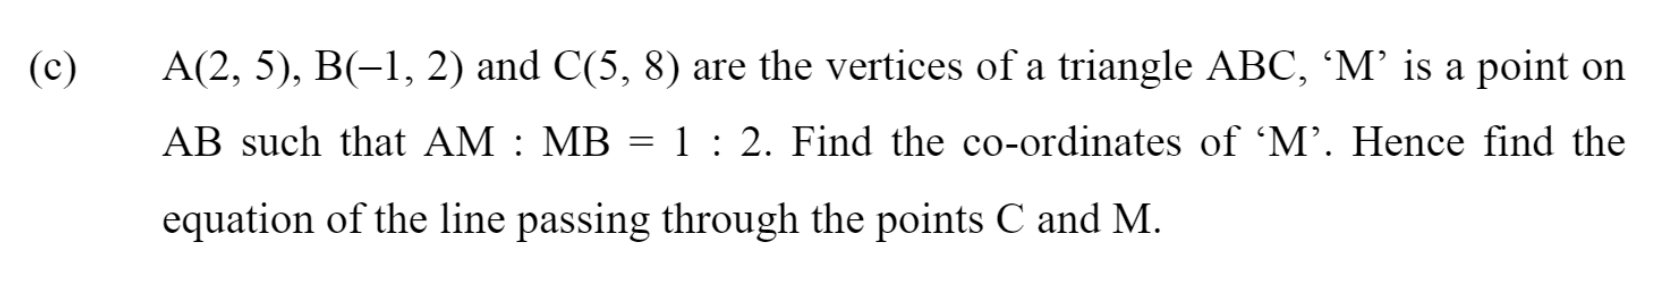
\includegraphics[width=0.49\textwidth]{prv1a.png}
\end{center}

\solution According to the question, $M$ is a point on the side $AB$ such that $$AM : MB = 1 : 2$$
 When the line segment AB is divided internally by C in the ratio $m:n$, from Section formula,\\
 we get the Coordinates of point C as,
\begin{align} \label{1}
\vec{C} = \myvec{\frac{mx2+nx1}{m+n}\\\\ \frac{my2+ny1}{m+n}}, where\\
     \vec{A}=\myvec{x1\\y1}, \vec{B}=\myvec{x2\\y2} \label{2}
\end{align}
From given data, Using \eqref{1} here, we get
\begin{align}
    \vec{M} &= \myvec{\frac{-1+4}{1+2}\\\\ \frac{2+10}{1+2}}\\  \label{3}
   &= \myvec{1\\4}
\end{align}\\\\ 
The equation of the line joining two points \myvec{a\\b} and \myvec{c\\d} is 
\begin{align}
    \myvec{y-b} = {\myvec{\frac{d-b}{c-a}}}\myvec{x-a} \label{5}
\end{align}
Here, the equation of the line joining points C\myvec{5\\8} and M\myvec{1\\4} will be
\begin{align}
    \myvec{y-4} = \myvec{\frac{8-4}{5-1}}\myvec{x-1} \label{6}
\end{align}
Simplified, we get the equation
\begin{align}
    \myvec{1 & - 1}\vec{x} + 3 &=0 
\end{align}
 which can also be represented as 
 \begin{align}
     x-y+3=0
 \end{align}
\subsection*{But, However,} On using \eqref{5}, we get\\
\begin{enumerate}
    \item The equation of the line joining $\vec{A}\myvec{2\\5}, \vec{B}\myvec{-1\\2}$ as $\myvec{1 & - 1}\vec{x} + 3 = 0$ \\\\
    
    \item and the equation of the line joining $\vec{B}\myvec{-1\\2}, \vec{C}\myvec{5\\8}$ as $\myvec{1 & - 1}\vec{x} + 3 = 0$ too.\\
\end{enumerate}

 This implies that $A,B,C$ points are `collinear' and lie on the line $x-y+3=0$ and Hence, given points $A,B,C$ don't form a triangle.\newline\\
Verified by plotting the graph of A,B,C and M points :
\begin{center}
  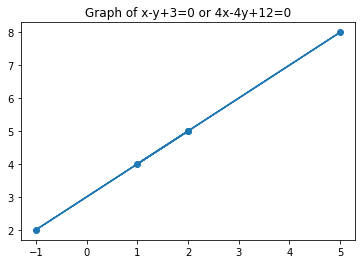
\includegraphics[scale=0.6]{prv1b.png}
\end{center}
    
\end{document}
